\documentclass[10pt,aspectratio=169]{beamer}
\usetheme{Madrid}
\usepackage{fontspec}
\usepackage{xeCJK}
\setCJKmainfont{Hiragino Sans GB}
\setCJKsansfont{Hiragino Sans GB}
\usepackage{booktabs}
\usepackage{xcolor}
\usepackage{tikz}
\usetikzlibrary{arrows.meta,positioning}
\usepackage{amsmath}
\definecolor{acc}{HTML}{2B5DD8}
\definecolor{good}{HTML}{1F9D6B}
\definecolor{warn}{HTML}{C77700}
\definecolor{bad}{HTML}{C0392B}
\setbeamercolor{structure}{fg=acc}
\setbeamercolor{palette primary}{bg=acc,fg=white}
\setbeamercolor{palette secondary}{bg=acc!80!black,fg=white}
\setbeamercolor{palette tertiary}{bg=acc!60!black,fg=white}
\setbeamercolor{title}{fg=acc}
\setbeamertemplate{navigation symbols}{}
\setbeamerfont{frametitle}{size=\large,series=\bfseries}
\newcommand{\hl}[1]{\textcolor{good}{\textbf{#1}}}
\newcommand{\wa}[1]{\textcolor{warn}{\textbf{#1}}}
\newcommand{\ba}[1]{\textcolor{bad}{\textbf{#1}}}
\newcommand{\sexec}{\sigma_{\mathrm{exec}}}
\newcommand{\schunk}{\sigma_{\mathrm{chunk}}}

\title[The Policy Inverts the Filter]{The Policy Inverts the Filter}
\subtitle{导数动作空间重塑的是探索，不是行为：故事、问题、形式化与实验计划}
\author{项目汇报 · 2026-09-08}
\date{论文初稿 v0.3（ICLR 形态）· \texttt{awesome\_robo\_ttt/paper}}

\begin{document}

\begin{frame}
\titlepage
\end{frame}

\begin{frame}{一句话}
\begin{block}{论点}
所有「导数 / 速度 / 低通」动作接口都是策略与执行器之间的同一族一阶滤波器
\[
c_t=\lambda\,c_{t-1}+s\,u_t .
\]
只要策略能看见滤波器状态 $c_{t-1}$（导数标签可辨识的必要条件），接口就是位置策略的\hl{精确重参数化}：
它不能改变意图轨迹，只能改变\textbf{加在输出上的扰动}（探索噪声、模型误差、适应修正）如何到达执行器。
\end{block}
\vspace{2mm}
\begin{columns}[T]
\column{0.48\textwidth}
\textbf{于是被反复宣称的收益变成：}
\begin{itemize}
\item 更好的 BC 先验：\hl{成立}，但来自「条件于上一步指令 + 目标归一化」
\item 有色探索噪声：\hl{成立}（双刃剑）
\item 更平滑的执行：\ba{只对扰动成立}，意图不变
\item 更易微调 / 更鲁棒：\ba{由执行端探索噪声决定}，与结构无关
\item 更安全的适应位点：\ba{不存在}（上游修正被策略抵消）
\end{itemize}
\column{0.48\textwidth}
\textbf{证据}：12 个训练配置、5 个评测轴、每格 3 评测 seed、主臂 5 训练 seed；
以及一套让我们自己的先导实验\ba{三次得出相反结论}的评价协议。
\vspace{2mm}

\textbf{形态}：负结果 + 设计指南（ICLR 分析型论文）。
\end{columns}
\end{frame}

\begin{frame}{问题：动作接口的主张为什么难比较}
\begin{columns}[T]
\column{0.52\textwidth}
\textbf{常见做法}：换一个动作参数化（速度、增量、加速度、低通），与\emph{一个}基线在\emph{同一个策略侧噪声} $\sigma$ 下比较。

\vspace{2mm}
\textbf{三个隐藏的混杂}：
\begin{enumerate}
\item 滤波器悄悄改变了\textbf{执行端}的探索噪声（增益 $s/\sqrt{1-\lambda^2}$），同 $\sigma$ 不等于同探索预算；
\item 「导数策略」需要重训先验并把滤波器状态放进观测，这两件事各自有独立效应；
\item 一个滤波器对意图和对扰动的作用完全不同，但通常只测其一。
\end{enumerate}
\column{0.46\textwidth}
\begin{block}{我们自己踩过的坑（先导实验）}
\begin{itemize}
\item 与同 $\sigma$ 孪生比：接口鲁棒性 \hl{+25 至 +37 pp}
\item 与默认 $\sigma$ 的原版比：\ba{原版 81\% vs 接口最高 46\%}
\item 「积分作用补偿增益」：补偿比实测 0.66 = 增益本身，\ba{没有积分}
\item 适应修正装在了积分器\ba{下游}，从未测过结构保护
\end{itemize}
\end{block}
每一条后来都成了协议里的一条对照。
\end{columns}
\end{frame}

\begin{frame}{形式化 I：一族滤波器，一个平面}
\centering
\begin{tikzpicture}[>=Latex, node distance=8mm, every node/.style={font=\small}]
\node[draw, rounded corners, minimum width=18mm, minimum height=8mm] (pi) {策略 $\pi$};
\node[draw, rounded corners, right=13mm of pi, minimum width=30mm, minimum height=8mm] (f) {$c_t=\lambda c_{t-1}+s\,u_t$};
\node[draw, rounded corners, right=13mm of f, minimum width=22mm, minimum height=8mm] (plant) {控制器 + 执行器};
\draw[->] (pi) -- node[above] {$u_t$} (f);
\draw[->] (f) -- node[above] {$c_t$} (plant);
\draw[->] (plant.south) -- ++(0,-5mm) -| node[pos=0.25, below] {观测 $o_t$} (pi.south);
\draw[->, dashed, bad, thick] (f.north) -- ++(0,5mm) -| node[pos=0.25, above] {\textcolor{bad}{$c_{t-1}$：滤波器状态可观测}} (pi.north);
\end{tikzpicture}

\vspace{3mm}
\begin{tabular}{lccc}
\toprule
接口 & $(\lambda,s)$ & DC 增益 $s/(1-\lambda)$ & 策略看见状态？\\
\midrule
原版（位置增量） & $(0,1)$ & 1 & 无状态 \\
低通 $\alpha$（原版先验 + 滤波） & $(\alpha,1-\alpha)$ & 1 & 否 \\
导数接口（重标注先验） & 任意，$s/(1-\lambda)>1$ & $>1$ & \ba{是（必需）} \\
纯积分 & $(1,s)$ & $\infty$ & 是 \\
\bottomrule
\end{tabular}

\vspace{2mm}
\small 导数标签 $u_t=(a_t-\lambda c_{t-1})/s$ 依赖 $c_{t-1}$，而 $c_{t-1}$ 不是机器人状态的函数：不放进观测，先验拟合相关 $\approx0$、成功率 0\%。
\end{frame}

\begin{frame}[shrink=8]{形式化 II：恒等式与四条推论}
\begin{block}{命题 1（可观测状态的接口是重参数化）}
把闭环重标注 $u_t=(a_t-\lambda c_{t-1})/s$ 代回滤波器：
\[
c_t=\lambda c_{t-1}+(a_t-\lambda c_{t-1})=a_t\qquad\text{（不触发裁剪时恒等）}
\]
复现标签的策略精确执行示教指令，对任意 $(\lambda,s)$；导数接口 $=$ 位置策略 $\pi(a_t\mid o_t,c_{t-1})$ 换到输出坐标 $(a_t-\lambda c_{t-1})/s$。
\end{block}
\begin{columns}[T]
\column{0.5\textwidth}
\textbf{(i) 意图不变}：执行 = 意图 + \emph{滤波后的}模型误差；接口最多比原版平滑到示教水平，不会更平滑。

\textbf{(ii) 输出被预白化}：标签 $=(a_t-\lambda a_{t-1})/s$；若示教是 AR(1)（系数 $\phi$），标签 lag-1 自相关
\[
\frac{(\phi-\lambda)(1-\lambda\phi)}{1+\lambda^2-2\lambda\phi}
\]
在 $\lambda=\phi$ 处为零、之上为负、之下为正：\textbf{训练前就在数据里}。
\column{0.5\textwidth}
\textbf{(iii) 上游修正是扰动}：缩放 $u$ 改变了输出到 $c$ 的映射，策略观测 $c$、在下一决策点把它抵消。

\textbf{(iv) 不可能性}：滤波器要么被观测（不能平滑意图），要么不被观测（导数标签不可辨识、位置先验失配）。\ba{平滑意图与可训练的导数先验互斥。}

\vspace{2mm}
\textbf{推论}：导数接口的先验优势只能来自「条件于 $c_{t-1}$」和「目标按 $1/s$ 缩放」，与积分无关。
\end{columns}
\end{frame}

\begin{frame}{形式化 III：滤波器对扰动做什么}
设 $\delta u_t$ 为加在输出上的任何东西（探索噪声、模型误差、适应修正）。
\begin{itemize}
\item \textbf{事实 1 谱整形}：白噪声 $\sigma^2$ 经滤波成 AR(1)，稳态 std $\ \sexec=s\sigma/\sqrt{1-\lambda^2}$；带限谱指数从 0 升到 2，$\lambda\approx0.7$ 对应粉噪 $\beta\approx1$。
\item \textbf{事实 2 有界传播}：$|\delta u|\le\Delta\Rightarrow|\delta c|\le s\Delta/(1-\lambda)$。
\item \textbf{事实 3 执行空间信任域}：$|c_t-c_{t-1}|\le(1-\lambda)C_{\max}+s$，与参数改了多少无关。
\end{itemize}
\begin{block}{策略真正「看得见」的噪声：块尺度}
策略每 $H=4$ 步重规划，能学着纠正的是一个块内累积的位移：
\[
\schunk=\sexec\sqrt{\textstyle\sum_{i,j<H}\lambda^{|i-j|}}
\quad=\;2\sigma\ (\text{白噪声})\;\;\text{或}\;\;3.5\text{--}3.9\,\sexec\ (\lambda\in[0.8,0.95]).
\]
同样的稳态方差，红噪声对策略「可见」得多。
\end{block}
\small 三条事实对低通与导数接口\textbf{完全相同}，只依赖 $(\lambda,s)$；由命题 1，它们约束扰动、不约束意图。事实 1 只对\textbf{上游}注入成立：适应修正装在哪一侧决定滤波器是否保护它。
\end{frame}

\begin{frame}{评价协议：四条对照，各配一个它避免的错误结论}
\begin{tabular}{p{0.30\textwidth} p{0.62\textwidth}}
\toprule
\textbf{对照} & \textbf{若缺失，本研究会得出的错误结论} \\
\midrule
C1 匹配 $\schunk$ 的孪生 \textbf{加} 最强原版基线 & 「接口比原版鲁棒 +25--37 pp」「原版用不起补偿」：其实孪生只是低噪声训坏的策略；原版默认 $\sigma$ 下 81\% vs 接口 $\le$46\% \\
C2 不可观测低通零假设（同事实 3 界） & 「接口更平滑」：低通在信任域上紧 4 倍、jerk 低 3 倍 \\
C3 机理必须配可反驳的直接测量 & 「积分作用补偿增益漂移」：补偿比 0.66 = 增益本身 \\
C4 上游 / 下游两侧注入 & 「适应享受结构界」：补偿装在下游，测的是策略的闭环耐受 \\
\bottomrule
\end{tabular}
\vspace{3mm}

\textbf{第五条来自图本身}：匹配探索预算必须匹配 $\schunk$ 而非 $\sigma$。先导实验匹配了 $\sigma$，实际比较的是 $\sexec$ 0.069 vs 0.030。
\end{frame}

\begin{frame}{实验设计：12 点 $\times$ 5 轴}
\begin{columns}[T]
\column{0.46\textwidth}
\textbf{管线}：robomimic Square · DPPO（扩散 MLP 先验 3000 epoch $\to$ PPO 200 itr，探索参数 $\sigma$）· OSC 20 Hz · 块长 4 · 400 步。

\vspace{1mm}
\textbf{点}（历史代号）：
\begin{itemize}\small
\item 原版 A ($\sigma$=.10)、E5 (.03)
\item 低通 (0.8,0.2)：B (.10)、F4 (.03)；重训+可观测：F5 (.03)、F7 (.10)，构成先验$\times\sigma$ 的 2$\times$2
\item 导数：E4 (0.9,1.0,.03)、F1 (0.9,0.3,.03)、F6 (0.9,0.3,\textbf{.07})、F2 (0.7,1.0)、F3 (0.95,0.5)、纯积分 E1
\end{itemize}
\textbf{五轴}：先验对齐 · RL 可训性 · 执行平滑（jerk、最大单步）· 部署鲁棒（增益 $\times$0.7、延迟 2、观测噪声）· 信号与适应（校准相关、恢复、被骗代价）。
\column{0.54\textwidth}
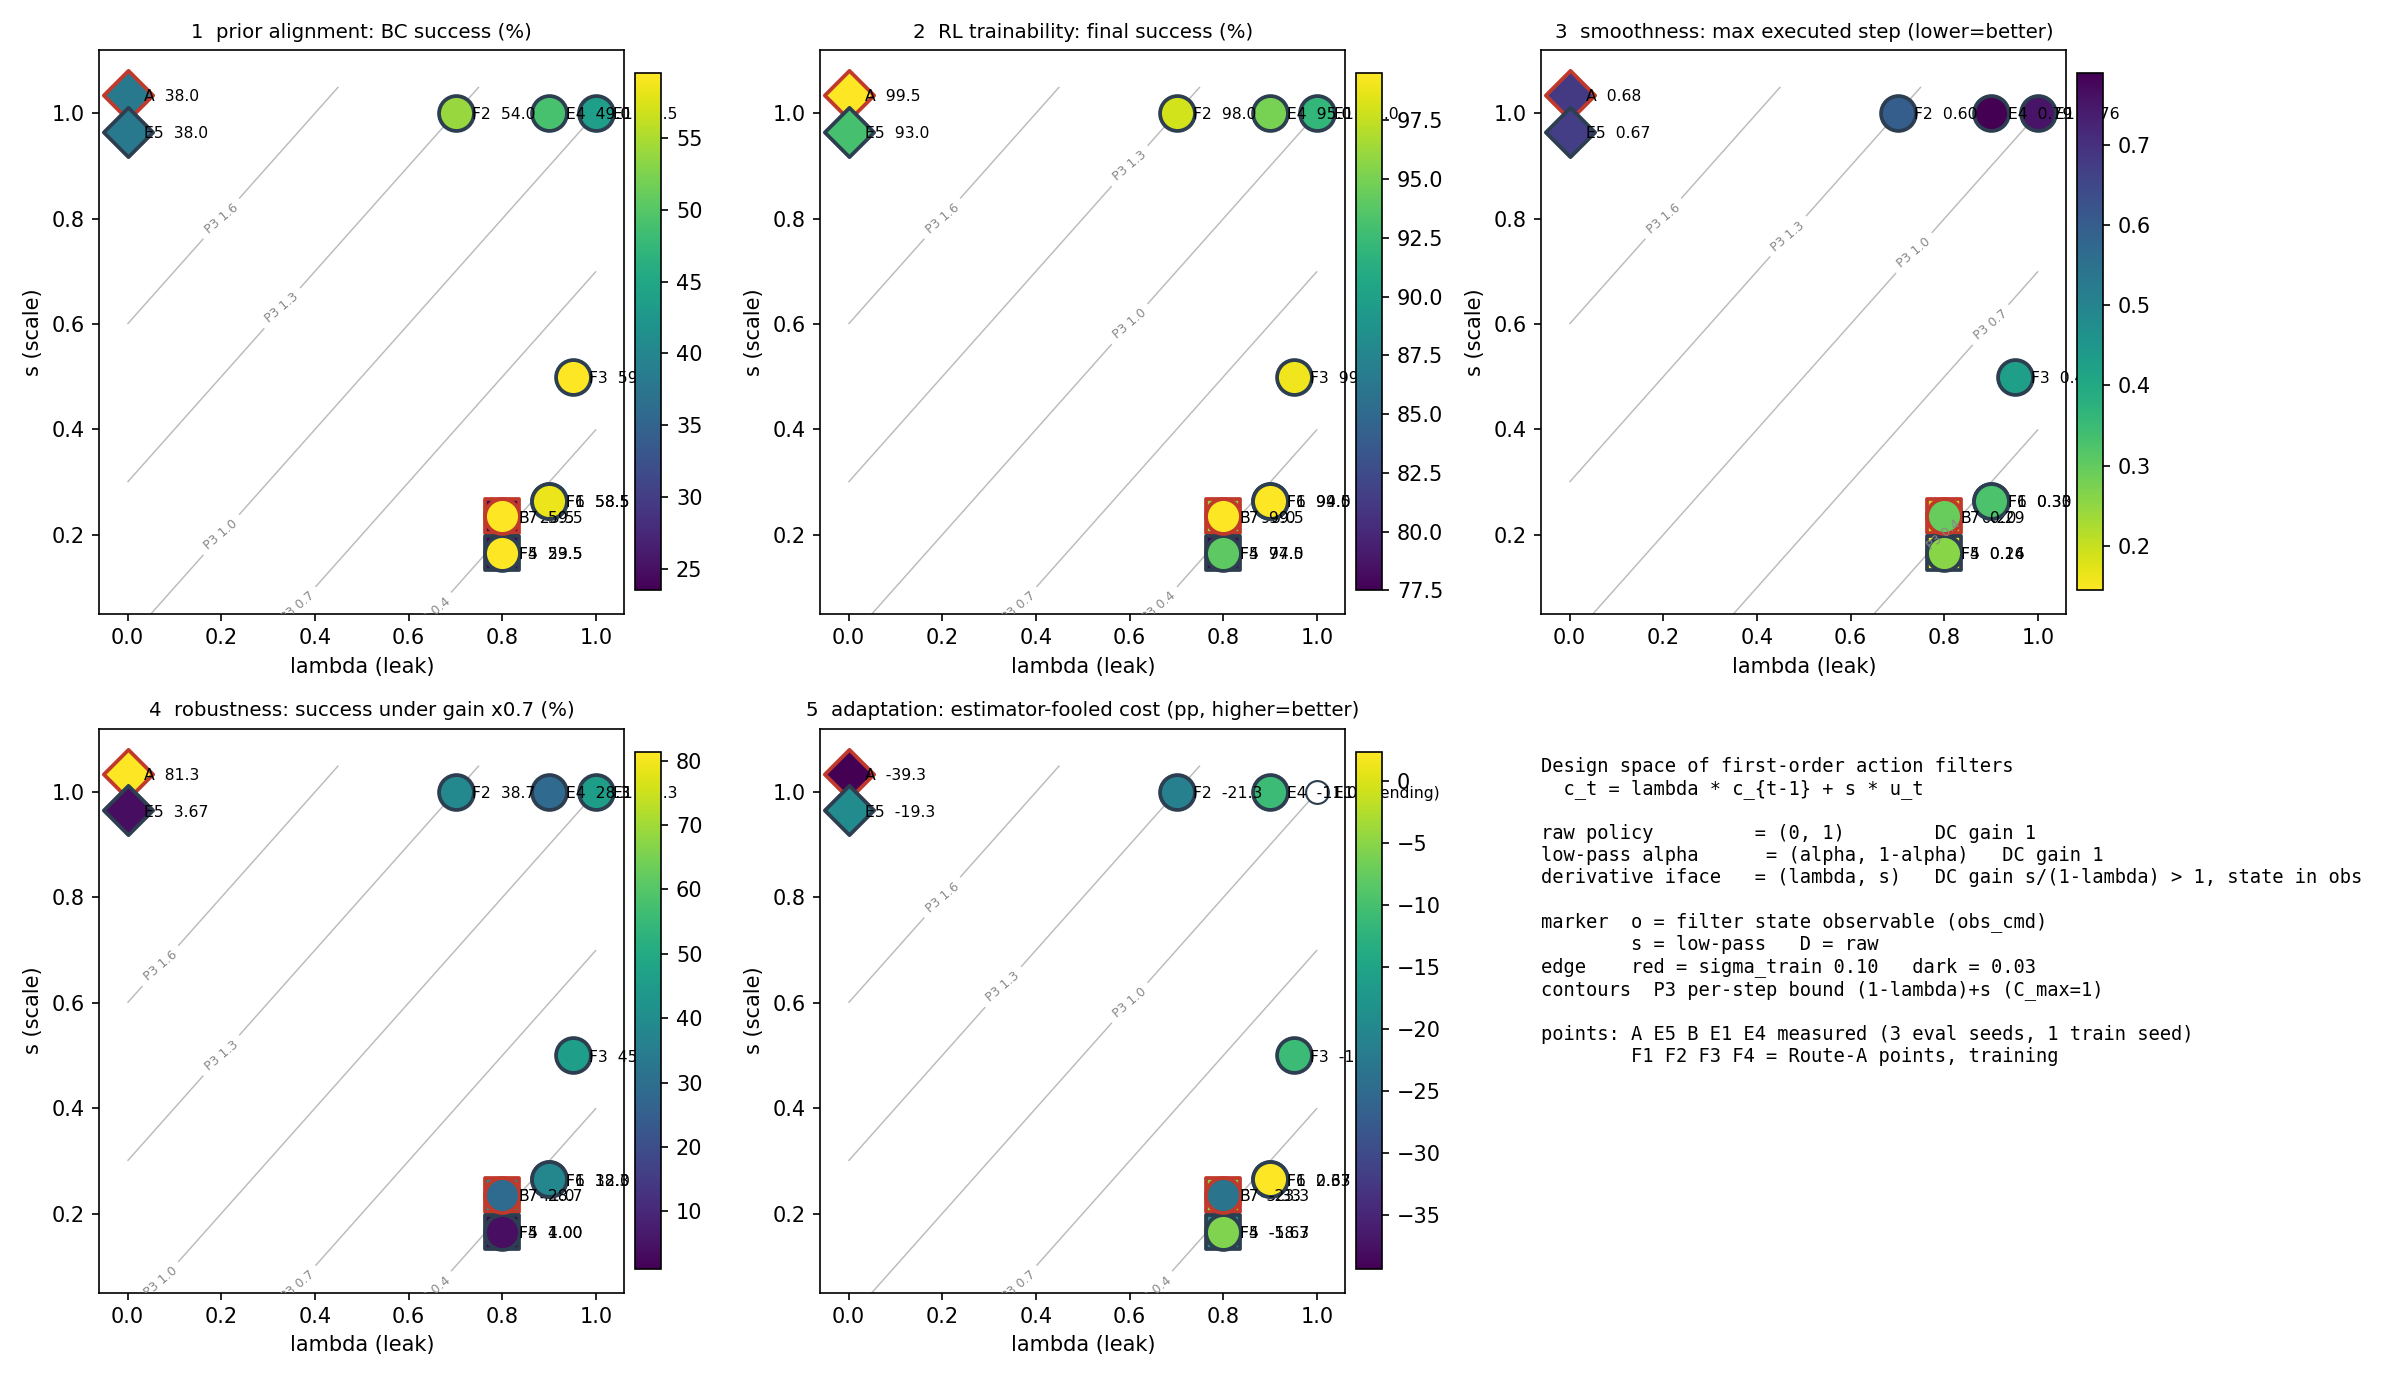
\includegraphics[width=\textwidth]{../figures/DS_map.png}
\end{columns}
\end{frame}

\begin{frame}[shrink=5]{结果 I：意图通道，先验、平滑、白化}
\begin{columns}[T]
\column{0.5\textwidth}
\textbf{先验随 $s$ 减小而变好}（与预注册方向相反）
\begin{itemize}
\item $(0.9,1.0)$ 49.0 $\to$ $(0.9,0.3)$ \hl{58.5}；$(0.95,0.5)$ 59.5；原版 38.0
\item 原因：$s=1$ 时标签 $|u|\approx0.07$，淹在扩散输出噪声底下；\textbf{目标归一化}
\item DC 增益无关：低通 $(0.8,0.2)$ + 重训 + 可观测（F5）= 59.5
\end{itemize}
\textbf{执行平滑 = 示教平滑}
\begin{itemize}
\item 示教：$\phi$=0.91、$\beta$=1.93、jerk 0.107
\item 可观测接口 jerk 0.07--0.13、$\beta$ 1.8--2.25 $\approx$ 示教
\item 原版 0.16--0.18（模型误差未滤）；\hl{不可观测低通 0.03}
\item 同滤波器同 $\sigma$：F4$\to$F5 jerk $\times$2.8，B$\to$F7 $\times$3.2
\end{itemize}
\column{0.5\textwidth}
\textbf{白化在数据里，不是 RL 学的}
\begin{center}\small
\begin{tabular}{lccc}
\toprule
$\lambda$ & 数据集标签 ac$_1$ & AR(1) 预测 & 微调后策略 \\
\midrule
0.7 & +0.35 & +0.35 & +0.40 \\
0.8 & +0.24 & +0.16 & +0.25 / 0.31 \\
0.9 & $-$0.08 & +0.01 & $-$0.14 / $-$0.11 \\
0.95 & $-$0.14 & $-$0.03 & $-$0.11 \\
\midrule
不可观测 B / F4 & -- & -- & +0.81 / +0.78 \\
\bottomrule
\end{tabular}
\end{center}
\small 符号规律由命题 1(ii) 预测。「导数接口更平滑」对\textbf{扰动}成立（随机 rollout 中 E4 的执行谱指数 2.1--2.5 vs 原版 0.9），对\textbf{意图}不成立。
\end{columns}
\end{frame}

\begin{frame}{结果 II：扰动通道，可训性与鲁棒性由执行端噪声决定}
\begin{columns}[T]
\column{0.58\textwidth}
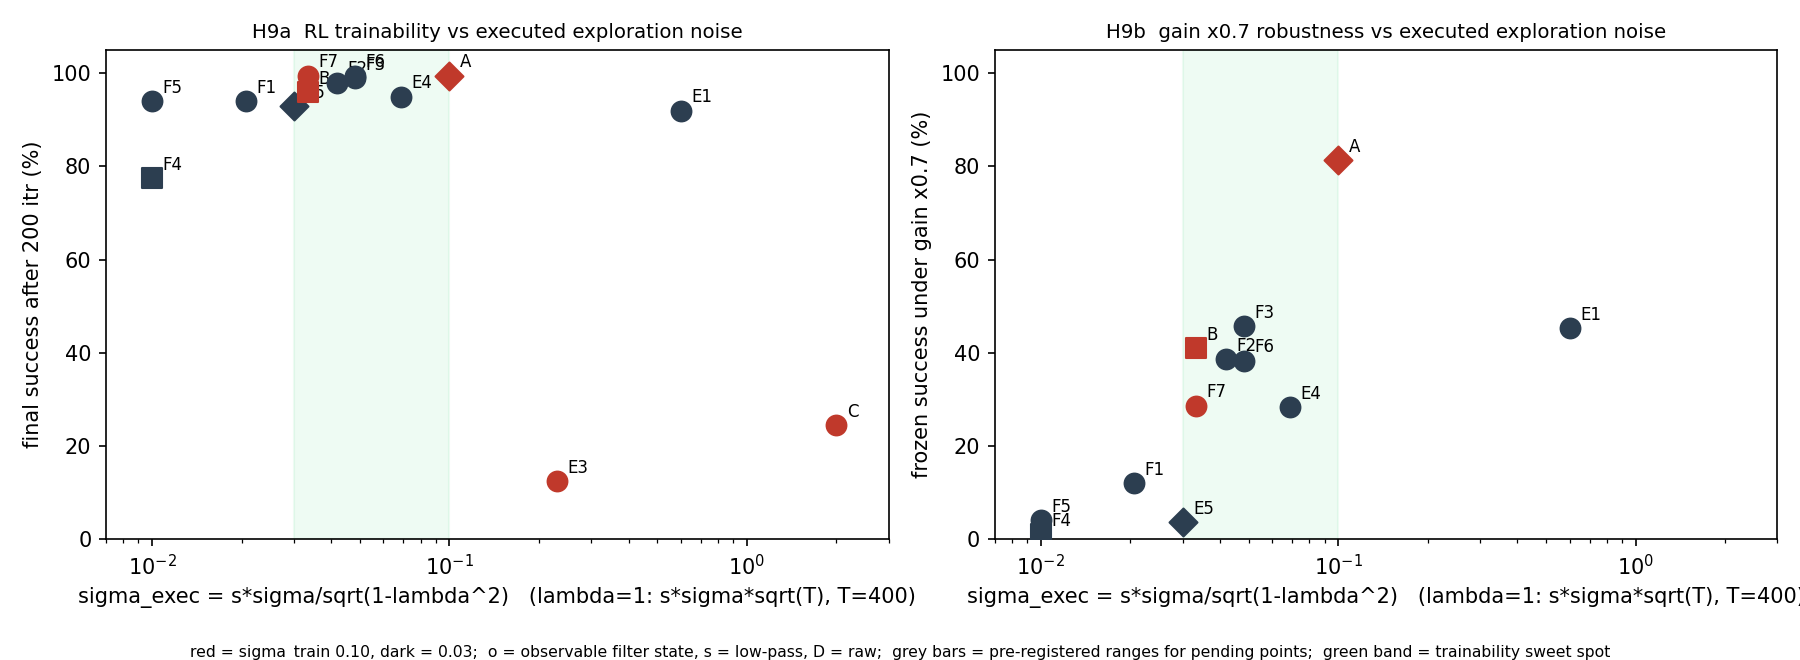
\includegraphics[width=\textwidth]{../figures/DS_h9.png}
\column{0.42\textwidth}
\begin{itemize}
\item \textbf{可训性倒 U}：$\sexec\in[0.02,0.10]$ 时 94--99.5\%；低通 $\sigma$=.03（0.010）77.5\%；导数接口 $\sigma$=.10（0.23）崩溃
\item \textbf{鲁棒性单调}：Spearman 0.76（10 点）/ \hl{0.92}（去 E4 的 9 点）
\item 块尺度解释了原版 $\sigma$=.03 为何与低通一样脆（3.7\% vs 1--4\%）：白噪声一个块内只累积 0.06，策略看不见
\item \ba{匹配执行噪声时没有接口赢过原版}；先导实验里的 +25 pp 是两个都在曲线之下的点之差
\item 训练 seed：接口 92.5$\pm$8.5 vs 原版 92.1$\pm$1.3（终值）；鲁棒性 25.9$\pm$7.5 vs 4.3$\pm$2.7
\end{itemize}
\end{columns}
\end{frame}

\begin{frame}{结果 III：适应位点与残差}
\begin{columns}[T]
\column{0.55\textwidth}
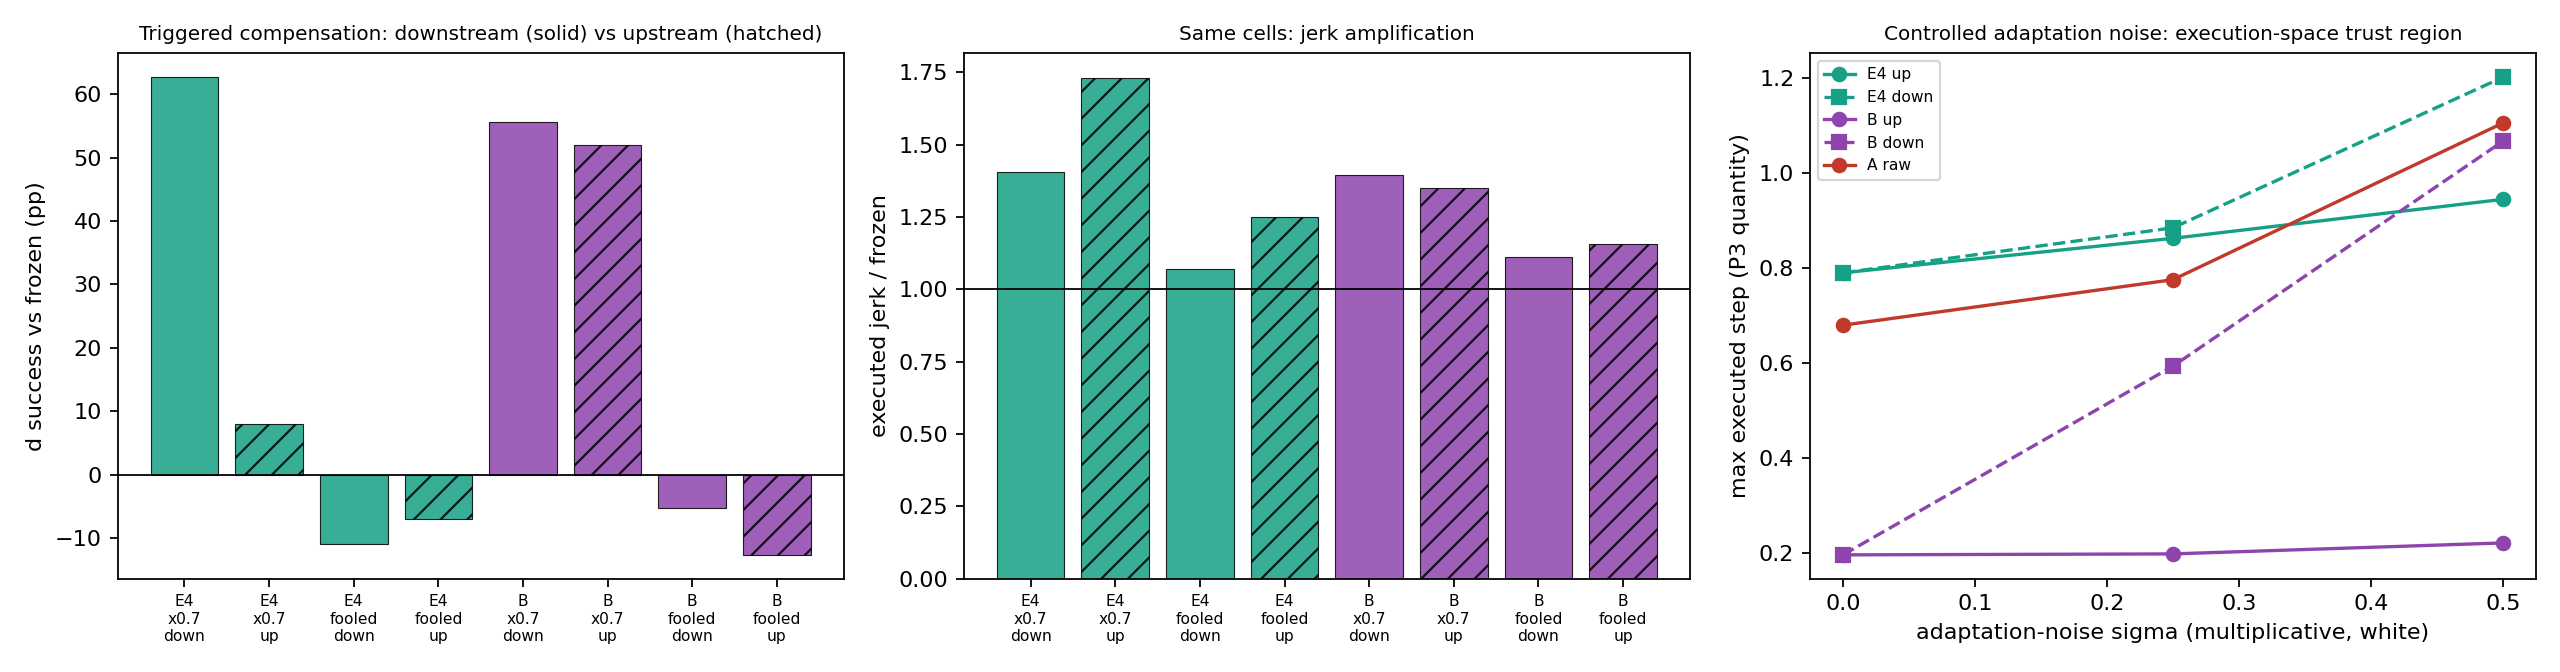
\includegraphics[width=\textwidth]{../figures/P1_upstream.png}
\column{0.45\textwidth}
\textbf{修正装在哪一侧决定一切}
\begin{itemize}
\item 下游（执行指令）：同一估计器恢复所有臂（原版 81$\to$99、接口 28$\to$91、低通 41$\to$97），测的是策略，不是接口
\item 上游（策略输出，事实 1 适用）：低通 92--93\% 与下游等效，适应噪声 jerk $\times$1.40 vs 下游 $\times$6.11，\hl{界是真的}
\item 可观测接口上游：\ba{27--36\%}（下游 87--91），且更抖 $\times$1.7--2.3：策略把缩放当扰动纠正（推论 iii）
\item 受保护的适应位点对可观测接口\ba{不存在}
\end{itemize}
\textbf{残差}：E4、F7 稳定低于噪声趋势（5 训练 seed）；已排除先验质量、seed、噪声尺度与颜色；工作假说：条件于自身指令历史的 copycat 型因果混淆，增益漂移恰好打断这条捷径。
\end{columns}
\end{frame}

\begin{frame}{对动作空间设计的五条规则}
\begin{enumerate}
\item \textbf{匹配执行端噪声 $\schunk$，不是 $\sigma$。} 同 $\sigma$ 的比较是不等探索预算的比较。
\item \textbf{平滑意图与导数先验二选一。} 不可观测滤波器平滑意图但标签不可辨识；可观测滤波器可训练但只平滑扰动。平滑主张要在确定性 rollout 上与同界低通比。
\item \textbf{归一化导数目标。} $s$ 决定标签相对生成模型输出噪声底的信噪比；归一化单位下 $s=1$ 是原接口最坏的一个选择。
\item \textbf{预期指令条件带来的漂移惩罚}，用历史丢弃检验。
\item \textbf{不要指望策略看得见滤波器时还有受保护的上游适应位点。}
\end{enumerate}
\begin{block}{把规则 1、3 用在原接口上：F6 $=(0.9,0.3)$ @ $\sigma$=0.07}
先验 +9.5 pp、终值 99.5、增益鲁棒 +10、观测噪声鲁棒 +11、最大单步 0.33 vs 0.79、被骗代价 +2 vs $-$11：除延迟外每个轴都优于原接口；
但零适应鲁棒性仍 38 vs 原版 81，正如规则 1 所预测。
\end{block}
\end{frame}

\begin{frame}{准备跑 / 在跑的实验}
\begin{tabular}{p{0.34\textwidth} p{0.40\textwidth} p{0.18\textwidth}}
\toprule
\textbf{实验} & \textbf{回答什么 / 预注册预测} & \textbf{状态} \\
\midrule
$\lambda=0$ 角点 2$\times$2：$(0,1)$、$(0,0.6)$ $\times$ \{可观测, 不可观测\}（仅 BC） & 先验提升分解：条件于 $c_{t-1}$ 占大头，缩放次之，仅重训 $\approx$ 原版 38 & \hl{在跑}（4 GPU，约 8 h） \\
BC 期历史丢弃（可观测点） & copycat 假说：E4 / F7 应回到 $\schunk$ 趋势线 & 待启动，约 1 天 \\
块长 $H\in\{1,4,8\}$，固定 $\sexec$ & $\schunk$ 的坍缩应变紧、$\sexec$ 的不变 & 待启动，约 2 天 \\
$\schunk$ 匹配的原版孪生 & 补上先导实验没做的那一组对照 & 待启动，约 1 天 \\
第二任务 robomimic Transport & 恒等式推论与噪声中介是否与任务无关 & 待启动，约 1 周 \\
主要点 5 训练 seed（现仅 E4 / E5） & 轴 3--5 的 seed 方差 & 视算力 \\
\bottomrule
\end{tabular}
\vspace{3mm}

\textbf{论文侧}：相关工作已按六条线补入；图的论文级排版（同坐标点标签）；附录含自我修正案例研究与估计器细节。

\textbf{时间}：角点结果明早；第二任务决定是否在本轮投稿内，这是投稿前最大的一个决定。
\end{frame}

\begin{frame}{局限与结论}
\begin{columns}[T]
\column{0.5\textwidth}
\textbf{局限}
\begin{itemize}
\item 一个任务（准静态插入）、一个仿真器、一个 RL 算法、低维观测
\item 多数点单训练 seed（主臂 5 个）
\item E4 / F7 低于趋势的残差已刻画、未解决
\item 平滑度是硬约束的任务（液体、易碎接触）可能给滤波接口不同的回报；由推论 (iv)，候选是不可观测低通而非导数接口
\end{itemize}
\column{0.5\textwidth}
\textbf{结论}
\begin{itemize}
\item 导数 / 速度 / 低通接口是同一族一阶滤波器
\item 策略看得见滤波器状态时，接口是位置策略的精确换坐标：\hl{重塑探索与适应噪声，不重塑行为}
\item 它买到的：更好的先验（条件 + 归一化）、有色探索
\item 它没买到的：意图平滑、微调、零适应鲁棒、受保护的适应
\item 图 + 恒等式 + 四条对照，让下一个动作空间提案更便宜地被检验、更难被高估
\end{itemize}
\end{columns}
\vspace{2mm}
\centering\small 稿件：\texttt{paper/main.pdf}（ICLR 2027 格式，11 页含附录）· 证据链：\texttt{proposal/CADI\_TTT\_PROPOSAL\_v2.md} §1.5--1.11 · 审稿：\texttt{paper/REVIEW\_iclr\_story\_v0.1.md}
\end{frame}

\end{document}
